\chapter[Statistická analýza dat]{B4M36SAN \\[1ex]\Large{Statistická analýza, modely a jejich hodnocení. Redukce dimenze. Shlukování.}}

\section{Redukce dimenze}

Při redukci dimenze chceme data dostat do nižší dimenze, např. kvůli vizualizaci nebo zmenšení při přenosu. Předpokladem je, že máme body $X = {x_i}$ z nějakého prostoru dimenze $D$. Předpokládáme, že $X$ leží aspoň přibližně na manifoldu dimenze $d < D$, kde $d$ je intrinsická dimenze.

Manifold je topologický prostor, na kterém můžeme měřit Euklidovské vzdálenosti s malou chybou. Manifoldem dimenze 1 je nějak zkroucená křivka v prostoru vyšší dimenze (ale ne osmička, protože uprostřed se kříží), manifoldem dimenze 2 je např. rovina zkroucená do rolády. Předpoklad toho, že data leží na manifoldu nižší intrinsické dimenze je důležitý proto, že kdyby na manifoldu neležela, pak nemá smysl redukovat dimenzi (protože se to nepovede).

Intrinsická dimenze popisuje, kolik proměnných je potřeba k popisu dat. Libovolný bod v $\mathbb{R}^3$ lze popsat třemi proměnnými, ale pokud víme, že leží na nějaké konkrétní přímce (nebo nějaké křivce), třeba na jedné z os, stačí nám proměnná jedna.

Výstupem Redukce dimenze je nový prostor nižší dimenze než $D$, a dvě mapovací funkce: z původního prostoru do toho redukovaného, a z redukovaného prostoru do toho původního.

\subsection{PCA - Principal Component Analysis}

PCA najde největší varianci a transformuje data tak, aby byla ve směru osy. Toho dosáhne tak, že diagonalizuje kovariační matici. Data nejprve \textit{posuneme do počátku}.

\begin{equation}
X = 
\left( \begin{array}{ccc}
1 & 1 & 1\\
1 & 2 & 1\\
1 & 3 & 2\\
1 & 4 & 3 \end{array} \right)
%
\sim
%
\left( \begin{array}{ccc}
0 & -1.5 & -0.75\\
0 & -0.5 & -0.75\\
0 & 0.5 & 0.25\\
0 & 1.5 & 1.25 \end{array} \right)
\end{equation}
Kovariační matici spočítáme tak, že na každou dvojici příznaků použijeme vzorec pro $\text{cov}(X, Y)$, a tím nám vznikne symetrická matice. Protože $E(X)$ všech příznaků je 0, tak se to dá zjednodušit na $C_X = \frac{1}{m}X^TX$.

\begin{equation}
\text{cov}(X,Y) = \frac{1}{n} \sum_{i=1}^n (x_i-E(X))(y_i-E(Y))
\end{equation}

Protože je kovariační matice symetrická, můžeme ji rozložit jako $C_X = P\Lambda P^{-1}$, kde $P$ má ve sloupcích vlastní vektory $C_X$ a $\Lambda$ je matice vlastních čísel. Protože $P$ je ortogonální, pak $P^{-1}=P^T$, a $P$ je zároveň transformační maticí, kterou hledáme.

\subsection{Kernel PCA}

PCA funguje dobře pro lineární data. Pokud máme data např. na kružnici, tak je PCA k ničemu. Chceme najít funkci $\Phi$, která data nejprve nějak upraví, aby šla lépe zpracovat (třeba $\mu_1 = x_1^2, \mu_2 = x_2^2$ pro kružnici, protože předpis kružnice je $x^2+y^2=1$).

Využijeme toho, že v PCA jsme pracovali s daty $X$ jen jako se skalárním součinem $X^TX$. Zvolíme kernel funkci $K$. Pokud chceme běžné PCA, pak bude rovna skalárnímu součinu: $K(x_i, x_j) = \langle x_i, x_j\rangle$. Můžeme ale zvolit jiné funkce (které musí splňovat nějaké vlastnosti) a pak můžeme postupovat stejně jako u PCA, jen počítáme $C_X = \frac{1}{m}K$.

Vhodnou kernel funkcí je např. RBF (radial basis function). KPCA funguje dobře i na nelineární manifoldy, a jeho složitost neroste s dimenzí dat (protože redukce dimenze se děje už v $K$). Nevýhodou je, že je těžké až nemožné získat funkci pro zpětnou transformaci dat.

\subsection{MDS - MultiDimensional Scaling}

Hlavní myšlenkou MDS je, že body, které jsou blízko sebe, mají zůstat blízko, a vzdálené body mají zůstat daleko od sebe. Řešíme úlohu, kde minimalizujeme stresovou funkci:

\begin{equation}
\text{stress}(T, f)=\sqrt{\frac{\sum_{i,j=1}^m(f(\delta_{ij})-d_{ij})^2}{\sum_{i,j=1}^m d_{ij}^2}}
\end{equation}

\noindent kde $T$ jsou data, $f$ je transformační funkce, a $d_{ij}$ a $\delta_{ij}$ jsou vzdálenosti v původním a novém prostoru.

Pro vhodný výpočet vzdálenosti na manifoldu můžeme použít funkci \textbf{Isomap}. V ní se sestaví graf (síť) nejbližších bodů, např. zohledněním okolí nebo nalezení $k$ nejbližších sousedů. Pak se spočítají euklidovské vzdálenosti mezi přímými sousedy, a vzdálenosti dalších bodů se získají jako délka nejkratší cesty grafem (součet euklidovských vzdáleností). 


\subsection{LLE - Locally Linear Embedding}

Každý bod vyjádříme jako lineární kombinaci sousedů, s nějakými váhami. Chceme, aby po transformaci zůstaly tyto váhy zachovány. Řešíme pak úlohu lineárního programování.

Výhodou LLE je, že jediným parametrem je počet sousedů, a je efektivní i pro velké datové sady. Nevýhodou je, že metoda není stabilní v řídkých oblastech, a pokud se do dat přidá nový bod, je potřeba vše spočítat znovu.

\subsection{t-SNE - t-Distributed Stochastic Neighbor Embedding}

Klade důraz na to, že malé vzdálenosti zůstanou podobné, u velkých povoluje větší změny. Vzdálenosti převedu na pravděpodobnosti (je pravdděpodobnější, že vytáhneme dva body, které jsou blízko sebe). Vzdálenost bodů $i$ a $j$ v původním prostoru bude nepřímo úměrná pravděpodobnosti $p_{ij}$, a v novém prostoru bude vzdálenost nepřímo úměrná pravděpodobnosti $q_{ij}$. Pak minimalizujeme Kullback-Leiblerovu divergenci:

\begin{equation}
S=KL(P||Q)=\sum_i\sum_{j\neq i} p_{ij}\text{log}\frac{p_{ij}}{q_ij}
\end{equation}

Ve slidech jsou obrázky, kde je vidět, že to dobře funguje na clusterování - třeba charakteristiky rukou psaných číslic tam jdou hezky rozdělit do skupin, protože důraz byl na to, aby podobné číslice zůstaly u sebe, a oddělení jednotlivých skupin nevadí.

\subsection{SOM - Self Organizing Map}
V sešitě o tom nic nemám a ze slidů to moc nechápu. Podle jednoho YT videa to vypadá, že se udělá síť s několika \textit{neurony} (zvolíme tolik neuronů, kolik očekáváme clusterů), a tu síť se snažíme napasovat na data:

\begin{enumerate}
\item Vybereme nějaký bod v datech
\item Najdeme nejbližší neuron, to je \textit{winner}, a síť posuneme/natáhneme tak, aby byl \textit{winner} blíž k vyubranému bodu
\item Jdeme na krok 1 a vybereme nový bod
\end{enumerate}

\noindent Na konci máme síť, kde každý neuron by měl být u jednoho clusteru dat. Je to dost podobné jako $k$-means.







\section{Shlukování}

Shlukování je zpracování dat, kdy se snažíme body rozdělit do $k>1$ tříd. Výsledkem je množina $\Omega = \{C_1, C_2, \dots, C_k\}$, kde $C_i$ jsou výsledné disjunktní shluky (množiny bodů). Vhodnou metodu budeme vybírat podle toho, jaká máme data: víme, kolik je shluků? Jak jsou shluky husté? Jaký mají shluky tvar?

\subsection{K-means}

\begin{enumerate}
\item Vyberu $k$ bodů z dat, klidně náhodně. Do nich umístím středy shluků.
\item U každého bodu v datech najdu, do kterého shluku patří (najdu nejbližší střed).
\item Každý střed posunu tak, aby ležel uprostřed svého shluku (tj najdu medián všech bodů, které přísluší k danému středu).
\item Opakuju body 2 a 3, dokud se středy mění.
\end{enumerate}

K-means vždycky skončí, protože součet vzdáleností bodů od středů se v kroku dva zmenší, a v kroku 3 zůstává stejný, a nemůžeme zmenšovat do nekonečna. Algoritmus může ale uváznout v lokálním minimu - to se obvykle řeší tak, že vybereme nejlepší výsledek z několika náhodně inicializovaných běhů.

Můžeme použít různé vzdálenostní funkce a bude to fungovat taky. Důležité je vybrat správné $k$. To se dá dělat tak, že spustím algoritmus pro různá $k$, a počítám nehomogenitu $W(k)$ (součet vzdáleností bodů od středů). Všechna $W(k)$ zakreslím do grafu a zvolím takové $k$, na kterém nehomogenita náhle klesla a dál už neklesá - graf tam vypadá jako pata. Další možností je $W(k)$ dále zpracovat a spočítat z něj Hartiganovo kritérium.

Variantou k-means je kernel k-means, kde nejprve body převedeme kernel funkcí a jejich vzdálenosti počítáme v jiném prostoru. Tím pak jdou shlukovat i data, která nejsou lineárně separovatelná.

\subsection{EM - Expectation Maximization}

Je složitý, vzorce nechápu, a proto sem dávám jen intuitivní popis. EM je hodně podobný algoritmu k-means co se týče postupu a kroků, ale liší se v tom, jak se body přiřazují do shluků. V k-means bylo přiřazení ostré: každý bod patří přesně do jednoho shluku, a shluk je definovaný svým středovým bodem. V EM jsou \textit{středy shluků} pravděpodobnostní rozdělení, která mají $\mu$ a rozptyly (v případě Gaussů). Pak nezjišťujeme, do kterého shluku bod patří, ale s jakou pravděpodobností patří do každého shluku (Expectation). V druhé fázi (Maximization) pak hledáme nové a lepší parametry shluků metodou MLE (Maximal Likelihood Estimation).

Výhodou EM oproti k-means je to, že na konci máme rozdělení, a můžeme generovat nové vzorky dat. Shluky taky můžou mít různé tvary.


\subsection{Hierarchické shlukování}

Data shlukujeme na základě podobnosti, nemusíme předem znát počet shluků. První možnost je začít s jedním shlukem a ten dělit na menší (to je sice efektivní, ale složité, a dál se tím nebudeme zabývat). Druhá možnost je umístit každý bod do vlastního shluku, postupně spojovat podobné shluky. Vzniká přitom strom - dendrogram, kde je vidět, jak se postupně shluky spojují, dokud nemáme jeden velký shluk.

\begin{figure}[ht!]
\centering
\includegraphics{SAN/img/dendrogram.png}
\end{figure}

Na základě dendrogramu se můžeme rozhodnout, kde shlukování zastavíme, udělat tam svislou čáru a tím určit počet shluků. Na obrázku máme svislé čáry dvě, jednou vznikne 6 shluků, druhou pouze dva shluky. \textit{Výška} v dendrogramu znázorňuje vzdálenost shluků

Pro tento typ shlukování je zásadní, jak počítáme vzdálenost shluků:
\begin{itemize}
\item \textbf{Single linkage} Vzdálenost shluků je rovna vzdálenosti dvou nejbližších bodů ve shlucích
\item \textbf{Complete linkage} Vzdálenost shluků je rovna vzdálenosti dvou nejvzdálenějších bodů ve shlucích
\item \textbf{Average linkage} Vzdálenost shluků získáme jako průměr vzdáleností všech dvojic bodů
\item \textbf{Centroid} Vzdálenost shluků získáme jako vzdálenost jejich středů
\end{itemize}

Vliv výpočtu vzdáleností shluků je patrný na obrázku níže, kde pracujeme s jednodimenzionálními daty: 2, 12, 16, 25, 29, 45.

\begin{figure}[ht!]
\centering
\includegraphics[width=\textwidth]{SAN/img/dendrogram-example.png}
\end{figure}

\subsection{Shlukování podle hustoty}

Předpokládáme, že shluky budou mít vyšší hustotu a budou odděleny místy, kde je hustota nižší. Výhodou takového algoritmu je, že nepotřebuje $k$ a umí najít i shluky, které jsou do sebe zamotané, třeba dvě spirály. Naopak problém je, pokud mají shluky různou hustotu.

Shlukování podle hustoty dělá algoritmus DBSCAN. Ten potřebuje dva parametry: velikost okolí a počet sousedů v husté oblasti. Body pak dělí do tří skupin: bod uvnitř shluku (má dost sousedů), hraniční bod (nemá dost sousedů, ale jeho přímí sousedi jsou uvnitř shluku) a bod mimo shluk (nemá dost sousedů, a nesousední s body uvnitř shluku). Výstupem jsou shluky a pak seznam bodů mimo ně.

\subsection{Spektrální shlukování}

Z dat vytvořím síť (graf) a postupně odebírám ty nejdelší hrany. Výsledkem je několik oddělených komponent (shluků). Pro jednoduchost budu pracovat s grafem, ve kterém jsou patrné dvě komponenty (jak se pracuje s body a ne z grafem je popsané níže).

\begin{figure}[ht!]
\centering
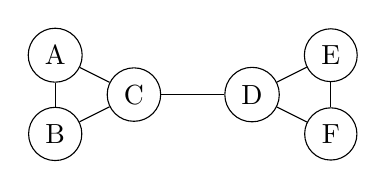
\begin{tikzpicture}
    \node[shape=circle,draw=black] (A) at (0,1) {A};
    \node[shape=circle,draw=black] (B) at (0,0) {B};
    \node[shape=circle,draw=black] (C) at (1, 0.5) {C};
    \node[shape=circle,draw=black] (D) at (2.5, 0.5) {D};
    \node[shape=circle,draw=black] (E) at (3.5, 1) {E};
    \node[shape=circle,draw=black] (F) at (3.5, 0) {F} ;

    \draw(A) to (B);
    \draw(B) to (C);
    \draw(A) to (C);
    \draw(D) to (C);
    \draw(D) to (E);
    \draw(D) to (F);
    \draw(E) to (F);   
\end{tikzpicture}
\end{figure}

Nejprve určím matici $S$, kde je jednička, pokud z vrcholu $i$ do vrcholu $j$ vede hrana. Protože je graf neorientovaný, bude matice symetrická. Pokud bychom nepracovali s grafem ale s body, tak matice $S$ bude \textit{similiarity}-matrix, kde počítáme blízkost bodů Gaussovým kernelem (čím bližší body, tím vyšší hodnota) a pak prahujeme podle nějaké konstanty. Tak jako tak vznikne symetrická matice.

Kromě matice $S$ sestavíme taky matici $D$, která bude mít na diagonále stupně vrcholů a jinak bude nulová (tedy je taky diagonální). Z nich spočítáme Laplacián grafu, $L = D - S$.

\begin{equation}
S = 
\left( \begin{array}{cccccc}
0 & 1 & 1 & 0 & 0 & 0\\
1 & 0 & 1 & 0 & 0 & 0\\
1 & 1 & 0 & 1 & 0 & 0\\
0 & 0 & 1 & 0 & 1 & 1\\
0 & 0 & 0 & 1 & 0 & 1\\
0 & 0 & 0 & 1 & 1 & 0\end{array} \right)
%
,
%
D = 
\left( \begin{array}{cccccc}
2 & 0 & 0 & 0 & 0 & 0\\
0 & 2 & 0 & 0 & 0 & 0\\
0 & 0 & 3 & 0 & 0 & 0\\
0 & 0 & 0 & 3 & 0 & 0\\
0 & 0 & 0 & 0 & 2 & 0\\
0 & 0 & 0 & 0 & 0 & 2\end{array} \right)
%
,
%
L = 
\left( \begin{array}{cccccc}
2 & -1 & -1 & 0 & 0 & 0\\
-1 & 2 & -1 & 0 & 0 & 0\\
-1 & -1 & 3 & -1 & 0 & 0\\
0 & 0 & -1 & 3 & -1 & -1\\
0 & 0 & 0 & -1 & 2 & -1\\
0 & 0 & 0 & -1 & -1 & 2\end{array} \right)
\end{equation}

K matici $L$ spočítáme vlastní čísla a vlastní vektory (postup je rozepsaný na webu v QR kódu), a vyjdou čtyři vlastní čísla a vektory:


\begin{figure}[H]
\centering
\begin{minipage}{0.15\textwidth}
\centering
\includegraphics[width=\textwidth]{SAN/img/spectral-clustering-qr}
\end{minipage} \hfill
\begin{minipage}{0.84\textwidth}

$\lambda_1 = 0, v_1 = (1, 1, 1, 1, 1, 1)$\\
$\lambda_2 \doteq 0.44, v_2 = (-1, -1, -0.56, 0.56, 1, 1)$\\
$\lambda_3 = 3, v_3 = (-1, 1, 0, 0, 0, 0)$\\
$\lambda_4 \doteq 4.56, v_4 = (-1, -1, 3.56, -3.56, 1, 1)$\\


\end{minipage}
\end{figure}

Teď jsou dva způsoby, jak z toho dostat shluky. Na přednášce jsme si říkali, že vektory dáme jako sloupce do matice $V$, a pak v řádcích té matice máme body. Na ně spustíme nějaké rychlé shlukování, třeba k-means. V přednáškách ze Stanfordu na to jdou ještě lépe, vezmou vektor odpovídající druhému nejmenšímu vlastnímu číslu (to nejmenší je nula a to je nuda), tedy v našem případě $v_2 = (-1, -1, -0.56, 0.56, 1, 1)$. Pak řeknou, že body, kterým přísluší záporné hodnoty (A, B, C) jsou jeden shluk a zbylé body jsou druhý shluk (D, E, F). Pokud chtějí víc clusterů, tak zpracovávají vektor $v_2$, někdy tam je těch úrovní zřetelných víc.


\section{Multivariátní analýza}

\subsection{ANOVA - Analýza rozptylu}

Zjišťujeme, jestli můžeme zamítnout hypotézu $H_0$: průměry ve všech skupinách dat jsou stejné (např. ženy, muži i děti mají stejnou výšku v cm). Mohli bychom to dělat třeba nepárovým t-testem na dvojici vzorků (párový t-test porovnává stejná data před a po, např. náladu lidí před vypitím kafe a po něm). Problém je, že pokud budeme dělat t-test pro každou dvojici skupin, tak to bude časově náročné pro hodně skupin, a taky tam bude víc chyb.

ANOVA předpokládá, že v každé skupině mají data normální rozdělení, že jsou nezávislá, a všechny skupiny mají stejný rozptyl. Zkoumáme vždy právě jednu proměnnou.

Zkusím to na třech třídách dat, $A = \{1, 2, 5\}, B = \{2, 4, 2\}, C = \{2, 3, 4\}$. Nulová hypotéza je, že všechny skupiny mají stejnou střední hodnotu. Všechno v postupu počítáme dvakrát, jednou mezi třídami (between) a pak uvnitř tříd (within). Názvy Ve slidech se to značí treat a error, což mě mátlo, a tak to sem psát nebudu.

Stupně volnosti jsou: $DF_{\text{between}} = k - 1 = 3-1 = 2, DF_{\text{within}} = N - k = 9 - 3 = 6$, kde $N$ je počet datových bodů, a $k$ je počet tříd. Pomocí stupňů volnosti najdeme tabulkovou $F$ hodnotu, $F_{\text{crit}} = 5.14$.

Spočítáme střední hodnota pro skupiny: $\mu_A=2.67,\mu_B=2.67,\mu_C=3$ a celkový průměr $\mu=2.78$. Počítáme \textit{Sum of Squares} ($SS$). Celkový $SS$ je součet vzdáleností všech bodů od střední hodnoty, a má dvě součásti: uvnitř skupiny a mezi skupinami. Sumy nejsou korektně značené, total se počítá pro všechna data, a within pro všechna data, ale odděleně po třídách.

\noindent $SS_\text{total} = \sum (x - \mu)^2 = (1-2.78)^2 + (2-2.78)^2 + (5-2.78)^2 + (2-2.78)^2 + (4-2.78)^2 + (2-2.78)^2 + (2-2.78)^2 + (3-2.78)^2 + (4-2.78)^2  = 13.6$

\noindent $SS_\text{within} = \sum (x - \mu_X) = (1-2.67)^2 + (2-2.67)^2 + (5-2.67)^2 + (2-2.67)^2 + (4-2.67)^2 + (2-2.67)^2 + (2-3)^2 + (3-3)^2 + (3-4)^2 = 13.34$

\noindent $SS_\text{between} = SS_\text{total} - SS_\text{within} = 13.6 - 13.34 = 0.23$

Dál počítáme \textit{rozptyly}:

\noindent $MS_\text{between} = \frac{SS_\text{between}}{DF_text{between}} = \frac{0.23}{2} = 0.12$

\noindent $MS_\text{within} = \frac{SS_\text{within}}{DF_text{within}} = \frac{13.34}{6} = 2.22$

Spočítáme $F$ hodnotu, $F=\frac{MS_\text{between}}{MS_\text{within}} = \frac{0.12}{2.22} = 0.05$

Protože $F<F_\text{crit}$, tedy $0.05 < 5.14$, tak nemůžeme nulovou hypotézu zamítnout, tedy je možné, že všechny skupiny mají stejnou střední hodnotu. F rozdělení je podíl dvou $\chi^2$ rozdělení.

Pokud by ANOVA nulovou hypotézu zamítla, tak pak by se třeba hodilo vědět, která ze skupin má odlišnou střední hodnotu. To nám ale ANOVA říct neumí, a musíme to zjistit jinak, třeba Tukeyho HSD testem. ANOVA umí pracovat pouze s jednou proměnnou, a pracuje s nezávislými měřeními.

\subsection{MANOVA}

Funguje podobně jako ANOVA, ale umožňuje víc náhodných veličin. Předpokladem je, že rozdělení jsou normální a mají napříč třídami stejné kovariační matice, jsou náhodně vzorkované atd, jako u ANOVy. Pro $p$ náhodných veličin vzniknou místo dvou hodnot $SS$ z ANOVy dvě matice $E$ a $H$ z $\mathbb{R}^p$. Pak ve vzorci není $(x - \mu)^2$, ale $(x_i - \mu_i)(x_j - \mu_j)$. Výsledek MANOVY se zpracuje Wilkovým lambda testem (nebo něčím jiným).







\section{Regrese}

\subsection{Lineární regrese}

Chceme data proložit přímkou (nebo rovinou). Předpokládáme, že data jsou lineární a že chyba od dat má normální rozdělení. I přes to, že jsou předpoklady nereálné, to dobře funguje. Pracujeme s modelem $Y = \beta_0 + \beta_1 X + \varepsilon$, kde $\beta$ jsou parametry, které hledáme, a $\varepsilon$ je chyba nebo šum.

Spočítáme RSS (Residual sum of squares) jako součet všech chyb: $RSS = \sum (y_i - \beta_0 - \beta_1x_1)^2$. RSS pak minimalizujeme, abychom dostali optimální parametry $\beta$.

Např. chceme proložit body: $[1, 3], [2,4], [3,5], [4, 4], [5,4], [6,5], [7,6], [8,7]$. Pro jednoduchost přejmenujeme parametry $\beta$, takže pracujeme se vztahem $y = a + bx + \varepsilon$. Vypočítáme $RSS = \sum (y_i - a - bx_i)^2 = (3-a-b)^2 + (4-a-2b)^2 + (5-a-3b)^2 + (4-a-4b)^2 + (4-a-5b)^2 + (5-a-6b)^2 + (6-a-7b)^2 + (7-a-8b)^2 = \cdots = 192 - 76a -370b + 8a^2  + 72ab + 204b^2$.

Tím máme RSS, a to chceme minimalizovat. Nejmenší hodnota bude tam, kde je nulová derivace (tam se křivka zvedá zase zpět nahoru).


\begin{minipage}{0.45\textwidth}
\begin{equation}
\begin{split}
\frac{\partial{RSS}}{\partial{a}} = 0 \\
-76 +16a +72b = 0 \\
16a + 72b = 76 \\
4a + 18b = 19 \\
a = \frac{19 - 18b}{4}
\end{split}
\end{equation}
\end{minipage} \hfill
\begin{minipage}{0.45\textwidth}
\begin{equation}
\begin{split}
\frac{\partial{RSS}}{\partial{b}} = 0 \\
-185+36a+204b=0 \\
36a+204b=185 \\
36\frac{19-18b}{4} + 204b = 185 \\
171 -162b+204b = 185 \\
42b = 14\\
b = \frac{1}{3}\\
a = \frac{19-\frac{18}{3}}{4} = \frac{13}{4}
\end{split}
\end{equation}
\end{minipage}

Dostali jsme parametry přímky: $y = \frac{x}{3} + \frac{13}{4}$. Vyznačené svislé čáry směrem k přímce jsou chyby $\varepsilon$, které jsme minimalizovali.

\begin{figure}[ht!]
\centering
\begin{tikzpicture}
\draw[help lines, color=gray!30, dashed] (0, 0) grid (8.9,8.9);
\draw[->, thick] (-0.2, 0)--(9,0) node[right]{$x$};
\draw[->, thick] (0,-0.2)--(0,9) node[above]{$y$};

\foreach \x/\y in {1/3,2/4,3/5,4/4,5/4,6/5,7/6,8/7}{
	\draw[color=red!60] (\x,\y)--(\x, 13/4+\x/3);
	\node at (\x,\y) {\textbullet};
}

% \foreach \Point in {(1, 3), (2,4), (3,5), (4, 4), (5,4), (6,5), (7,6), (8,7)}{
%     \node at \Point {\textbullet};
% }

\draw (-0.2, 3.183)--(8.9, 6.2167);

\end{tikzpicture}
\end{figure}

Jakmile máme parametry, tak můžeme měřit jejich chybu $SE$ pro každý z parametrů zvlášť, nebo RSE (residual standard error), což je odhad $\sigma$. Z hodnot $SE$ můžeme získat \textit{confidence intervaly}, které nám říkají, že s pravděpodobností $1-\alpha$ bude hodnota parametru ležet uvnitř toho intervalu. $SE(\beta_1)^2 = \frac{\sigma^2}{\sum_{i=1}^m(x_i-\bar{x})^2}$, kde jako $\sigma^2$ můžeme použít odhad $\sigma^2 = \frac{RSS}{m-2}$.

Testování hypotéz: Testujeme $H_0$, že není vztah mezi $X$ a $Y$, tedy $H_0: \beta_1 = 0$. Použijeme t-statistiku: $t = \frac{\beta_1 - 0}{SE(\beta_1)}$, kde za $\beta_1$ dosadíme parametr odhadnutý lineární regresí (a mně se nad něj nechce psát pořád stříšku). Má to $m-2$ stupně volnosti.

K hodnocení přesnosti modelu můžeme použít $R^2$, které nám říká, jaká část rozptylu v datech je vysvětlená modelem. $TSS = \sum_{i=1}^m(y_i - \bar{y})^2$ je celkový součet čtverců (vzdálenost od střední hodnoty), $RSS = \sum_{i=1}^m(y_i - \hat{y}_i)^2$ je vzdálenost bodů od odhadů. Pak $R^2 = \frac{TSS - RSS}{TSS}$.

Pokud chceme pracovat s vícedimenzionálním vstupem, přidáme další parametr beta:  $Y = \beta_0 + \beta_1 X_1 + \beta_2 X_2 + \varepsilon$. Pokud máme pocit, že se různé vstupy ovlivňují, např. zisk v závislosti na reklamu v televizi a reklamu v rozhlase, tak můžeme přidat ještě jeden parametr: $Y = \beta_0 + \beta_1 X_1 + \beta_2 X_2 + \beta_3 (X_1 X_2) + \varepsilon$ a pak zjišťujeme, které $\beta$ je nejvýznamnější.

\paragraph{Ridge regression}
Neminimalizujeme jen $RSS$, ale $RSS + \lambda\sum\beta_i^2$, tedy penalizujeme velká $\beta$, a parametr $\lambda$ určuje, jak přísně. To vede k tomu, že parametry $\beta$ budou co nejnižší, a tedy neužitečné proměnné se skoro nepoužijí ($\beta$ bude nula). Než se na datech spustí ridge regression, je vhodné data standardizovat (ve slidech je na to složitý vzorec, ale předpokládám, že to prostě od dat odečte střední hodnotu, aby byly v průměru na nule). Vhodný parametr $\lambda$ najdeme třeba cross-validací.

\paragraph{Lasso regression} Funguje stejně jako ridge regression, ale minimalizuje $RSS + \lambda\sum|\beta_i|$, tedy ne druhé mocniny. Tím budou koeficienty u neužitečných prediktorů nejen malé, ale dokonce nulové, a budeme je moct úplně zahodit.

\subsection{Nelineární regrese}

\paragraph{Polynomiální regrese} Pracujeme s polynomem nějakého daného stupně (to můžeme určit cross-validací), pak máme $Y = \beta_0 + \beta_1 X + \beta_2 X^2 + \cdots + \varepsilon$ a pokračujeme stejně jako u lineární regrese.

\paragraph{Krokové funkce} Rozdělíme $X$ na menší intervaly a v každém vybereme jako výsledek jednu konstantní hodnotu (třeba střední hodnotu). 

\begin{figure}[ht!]
\centering
\includegraphics[width=0.8\textwidth]{SAN/img/splines.png}
\end{figure}

\paragraph{Splines} Rozdělíme $X$ na menší intervaly, hraniční body mezi nimi jsou uzly. Hledáme polynomy takové, aby uvnitř intervalů co nejlépe seděly na datech, a v uzlech měly shodnou hodnotu  (a ideálně i derivaci, aby na sebe navazovaly). Na obrázku jsou ty samé body jako předtím proloženy dvěma parabolami s uzlem v bodě 3.5, a to tak, že v tomto bodě mají stejnou hodnotu a první derivaci.

\begin{figure}[ht!]
\centering
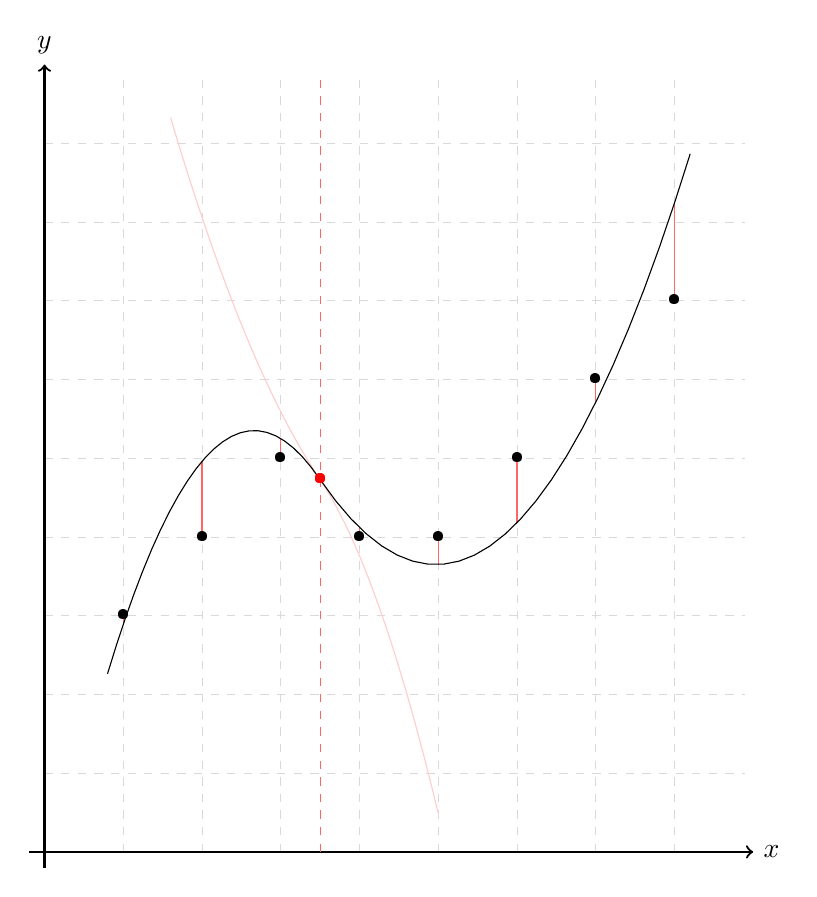
\begin{tikzpicture}
\draw[help lines, color=gray!30, dashed] (0, 0) grid (8.9,9.9);
\draw[->, thick] (-0.2, 0)--(9,0) node[right]{$x$};
\draw[->, thick] (0,-0.2)--(0,10) node[above]{$y$};

\foreach \x/\y in {1/3,2/4,3/5}{
	\draw[color=red!60] (\x,\y)--(\x, {(-0.89 * (\x) ^ 2 + 4.74 *\x + -0.96)});
	\node at (\x,\y) {\textbullet};
}

\foreach \x/\y in {4/4,5/4,6/5,7/6,8/7}{
	\draw[color=red!60] (\x,\y)--(\x, {(0.5 * (\x) ^ 2 + -4.97 *\x + 16)});
	\node at (\x,\y) {\textbullet};
}

\node[color=red] at (3.5, {(0.5 * (3.5) ^ 2 + -4.97 *3.5 + 16)}) {\textbullet};


\draw[color=red!20] plot[domain = 3.5:5] ({\x}, {(-0.89 * (\x) ^ 2 + 4.74 *\x + -0.96)});
\draw[color=red!20] plot[domain = 1.6:3.5] ({\x}, {(0.5 * (\x) ^ 2 + -4.97 *\x + 16)});

\draw plot[domain = 0.8:3.5] ({\x}, {(-0.89 * (\x) ^ 2 + 4.74 *\x + -0.96)});
\draw plot[domain = 3.5:8.2] ({\x}, {(0.5 * (\x) ^ 2 + -4.97 *\x + 16)});


\draw[color=red!60, dashed] (3.5, 0) to (3.5, 9.9);
\node[color=red] at (3.5, {(0.5 * (3.5) ^ 2 + -4.97 *3.5 + 16)}) {\textbullet};

\end{tikzpicture}
\end{figure}

Jak určit, kde budou uzly a kolik jich bude? Můžeme zvolit nějaké $k$ a pak uzly rozmístit rovnoměrně nebo podle kvantilů. Funkce mezi různými uzly můžou být různé - např. uprostřed dat můžeme volit paraboly, a na kraji dat přímky (lineární regresi), aby to bylo na krajích stabilnější (polynomy rychle vyjedou někam pryč). 

\paragraph{Lokální regrese} Hlavní myšlenka je, že ačkoliv data nejsou rozhodně lineární, tak v lokálním měřítku nám lineární odhad bude stačit. Vybíráme jen malé intervaly a na nich děláme po částech normální lineární regresi. Přitom interval nemusí být ostrý - můžeme si vzít nějakou kernel funkci a pomocí ní nějak pravděpodobnostně určovat, nakolik bod do toho \textit{intervalu} patří.


\subsection{Logistická regrese}

Logistická regrese rozděluje data do tříd, nebo přesněji, určuje, s jakou pravděpodobností bod patří do dané třídy. Nejčastěji se dělá pro dvě třídy. Mohlo by se zdát, že stejnou úlohu by zvládla i lineární regrese, ale ta není vhodná - pokud nás zajímá pravděpodobnost, tak bude linreg dávat nesmyslné hodnoty mimo [0, 1], a pokud jsou v datech outlieři, tak se to celé může zvrtnout. Proto do dat nedáváme lineární přímku, ale \textit{sigmoidu}:

\begin{figure}[ht!]
\centering
\begin{tikzpicture}
\draw[help lines, color=gray!30, dashed] (0, 0) grid (10.5,4.5);
\draw[->, thick] (-0.2, 0)--(11,0) node[right]{$x$};
\draw[->, thick] (0,-0.2)--(0,5) node[above]{$y$};

% e = 2.718
\draw[color=red!20] plot[domain = 0:10.3] ({\x}, {4*(2.718 ^ (\x - 5.3)/(1 + (2.718 ^ (\x - 5.3)))});


\draw[color=red!60, dashed] (5.3, 0) to (5.3, 4.5);
\node[color=red] at (5.3, 2) {\textbullet};

\foreach \x in {1, 2, 2.5, 3, 6}{
	\node[Green4] at (\x,0) {\textbullet};
}

\foreach \x in {5, 7, 8, 9, 10}{
	\node[blue] at (\x,4) {\textbullet};
}
\end{tikzpicture}
\end{figure}

Klíčový vztah pro pochopení logistické regrese je poměr pravděpodobností. V angličtině se tomu říká \textit{odds}, tady tomu budu říkat \textit{šance}. Šance je poměr pravděpodobností, že jev nastane vs že nenastane. Pokud se snažím na kostce hodit šestku, je pravděpodobnost úspěchu $p=1/6 \doteq 0.167$ a pravděpodobnost neúspěchu $p = 5/6 \doteq 0.833$. Šance na úspěšný hod je v tomto případě $s = \frac{1/6}{5/6} = 1/5 = 0.2$, ale lépe je to vyjádřit slovně, tedy \textit{jedna ku pěti}.

Nás bude v logistické regresi zajímat, jak se šance mění. To nám ukazuje funkce \textit{logit}, která je vlastně přirozeným logaritmem šancí. Zajímá nás úsek od 0 do 1, kde je funkce rostoucí, v krajních bodech není definovaná a vypadá docela podobně jako tangens. Pokud řekneme, že máme dvě třídy, 0: jev nenastal a 1: jev nastal, které odhadujeme na základě nějakých dat $d$, pak logit svazuje nějakou pravděpodobnost $p$ s hodnotou dat $d$. Praktičtější je inverzní logit, ten nám řekne jaká je pravděpodobnost, že jev nastal, na základě dat $d$. Protože logit nabýval na intervalu (0, 1) hodnoty z $(-\infty, \infty)$, tak inverzní logit je definovaný všude, a to se hodí.

\begin{equation}
\begin{split}
logit(p)=ln(\frac{p}{1-p})\\
log_e(\frac{p}{1-p}) = d\\
\frac{p}{1-p} = e^d\\
p = (1-p)e^d\\
p = \frac{e^d}{1+e^d}\\
P(d) = \frac{e^d}{1+e^d}
\end{split}
\end{equation}

Tím máme funkci $P$, která nám pro pozorovaná data řekne, s jakou pravděpodobností jev nastal. Navíc předpokládáme lineární závislost mezi daty a logaritmem šance (protože to je nejjednodušší a funguje to), tedy $d = ax + b$, kde $x$ je skutečně naměřená hodnota. Pak pravděpodobnost, že při této hodnotě nastal jev, je $P(x) = \frac{e^{ax+b}}{1+e^{ax+b}}$.

Koeficienty $a$ a $b$ najdeme metodou MLE (maximum likelihood estimation), tedy snažíme se vybrat takové parametry, aby naměřená data byla co nejpravděpodobnější. Budeme maximalizovat hodnotu $L$:

\begin{equation}
L(a, b) = \prod_{i, y_i = 1}P(x_i)\cdot\prod_{i, y_i = 0}(1 - P(x_i))
\end{equation}

Pro data výše, kde máme v třídě 0 hodnoty 1, 2, 2.5, 3 a 6 a ve třídě 1 hodnoty 5, 7, 8, 9 a 10, vyjdou nejlépe parametry $a=1, b=-5.3$. Tomu odpovídá funkce $P$ nakreslená v grafu červeně. Hraniční bod v této situaci je 5.3 - hodnoty vyšší než 5.3 pravděpodobně patří do třídy 1, ostatní do třídy 0. Model se dá taky použít ke zjištění, s jakou pravděpodobností patří bod do třídy. Třeba bod 7 patří do třídy 1 s pravděpodobností $P(7) = \frac{e ^{(7 - 5.3)}}{(1 + (e ^{(7 - 5.3))})} = 0.845$.

Logistická regrese jde dál upravit, aby pracovala s více než dvěma třídami, ale to tu ukazovat nebudu.


\subsection{Discriminant Analysis (LDA, QDA)}

Separuje datové třídy tím, že najde \textit{discriminant score} $\delta$, které se počítá z parametrů (Gaussovských) rozdělení. Vznikne rozhodovací hranice, která je buď přímkou (pak šlo o LDA, linear discriminant analysis), nebo křivkou (pak šlo o QDA, quadratic discriminant analysis).

\begin{figure}[ht!]
\centering
\includegraphics[width=0.7\textwidth]{SAN/img/lda-qda.jpg}
\end{figure}

Diskriminant je $\delta_k(x) = x\frac{\mu_k}{\sigma^2} - \frac{\mu_k^2}{2\sigma^2} + log(\pi_k)$, kde $\sigma_k$ je směrodatná odchylka ve třídě $k$, $\mu_k$ je střední hodnota ve třídě $k$, a $\pi_k$ je pravděpodobnost výskytu třídy $k$ v datech. Funguje to i na víc než 2 třídách, pak musí mít společnou kovariační matici.

Pravděpodobnost získáme z diskriminantu jako $P(Y=k|X=x) = \frac{e^{\delta_k(x)}}{\sum_{l=1}e^k{\delta_k(x)}}$. LDA funguje dobře, pokud máme málo dat a data jsou dobře separovatelná.




\section{Robustní statistika}

Chceme, aby výsledek našeho odhadu nebyl pokažen outliery nebo špatným předpokladem rozdělení. Zápisky i slidy jsou dost stručné, takže jen v bodech různé způsoby hodnocení odhadových metod:

\begin{itemize}
\item \textbf{Breakdown point}: největší možný podíl dat, který můžeme měnit, než to úplně znehodnotí odhad. U aritmetického průměru je Breakdown Point 0\%, protože jen jeden bod dokáže výsledek posunout úplně jinam. U mediánu je potřeba změnit 50\% dat.
\item \textbf{Influence Function}: dá se počítat přímo z dat (říká wikipedie), ale ve slidech je jiný druh. V něm se počítá, jaký vliv má na výsledek nějaké funkce změna dat v bodě $x$ o hodnotu $\varepsilon$. Na vstupu není celý dataset.
\item \textbf{ARE} - Asymptotic relative efficiency: Kromě správnosti odhadu měříme i to, jak často se mění, tedy vlastně rozptyl odhadů. ARE je vlastně podíl rozptylů pro dvě různé metody odhadu.
\end{itemize}

\paragraph{Odhady polohy} Snažíme se zjistit \textit{střed dat}, tedy třeba střední hodnotu, to jde dělat více metodami. Názorně to je vidět na ukázce dat: $\{-39.61, -26.29, -1.07, -0.92, -0.85, -0.16, 0.93, 1.91, 2.18, 133.65\}$.

\begin{itemize}
\item \textbf{Průměr}: Použijí se všechny hodnoty, vyjde 6.97. Průměr je ideální, pokud vzorky odpovídají normálnímu rozdělení.
\item \textbf{Medián}: Použijí se prostřední dvě hodnoty, tedy -0.85 a -0.16, a výsledek je -0.51.
\item \textbf{q\% trimmed}: Odstaníme daný podíl dat z obou stran, na \textit{prostředku} spočítáme průměr. Pokud odebereme 2 body z každé strany, vyjde výsledek -0.41.
\item \textbf{q\% windsorized}: Krajní body neodstraníme, ale nahradíme je za poslední hodnotu, kterou ještě použijeme. Se stejným $q$ jako v minulém bodě dostaneme data $\{-1.07, -1.07, -1.07, -0.92, -0.85, -0.16, 0.93,$ $1.91, 1.91, 1.91\}$, a z nich je průměr 0.33.
\item \textbf{Hodges-Lehman}: Data zpracováváme po dvojicích, spočítáme průměr pro každou dvojici, a z těchto průměrů vybereme medián, vyjde -0.03.
\end{itemize}

\paragraph{Robustní regrese} U lineární regrese jsme předpokládali, že chyby $\varepsilon$ mají normální rozdělení, a jako ztrátovou funkci jsme používali $(y-\bar{y})^2$. Pokud jsou chyby z jiného rozdělení, mění se i ztrátové funkce (může použít absolutní hodnotu, Huberovu fci, Hampelovu fci, nejmenší medián atd, ve slidech jich je hodně). Pak už se to optimalizuje daleko hůř.

\paragraph{Odhady rozptylu}
\begin{itemize}
\item \textbf{Směrodatná odchylka vzorku}: $\sigma^2 = 1/n\sum_{i=1}^n (x_i - \bar{x})^2$, kde $\bar{x}$ je průměrná hodnota vzorků (a někde je ve jmenovateli dokonce $n-1$, ale nevím, čím se to řídí).
\item \textbf{Mediánová odchylka}: $\text{MAD} = \text{med}\{|x_i - \text{med}\{x_i\}|\}$
\item $S_n$: Tohle je prý nejlepší a měli bychom to v praxi používat. $S_n = \text{med}_i \{\text{med}_j |x_i - x_j|\}$
\end{itemize}

\paragraph{Výpočet korelace} Korelace se počítá různě: Pearsonova korelace, Spearmanova korelace, Kendallova korelace. Každá má trochu jiný vzorec, a ani jeden sem přepisovat nebudu, stejně si to nebudu pamatovat. Kendallova korelace je nerobustnější, ale je pomalá - počítám, kolik z párů má \textit{shodu}, kde shoda tam je, pokud $x_i > x_j$ a zároveň $y_i > y_j$ (a to samé pro obě $<$). Zajímá mě počet shod mínus počet neshod.

\paragraph{Neparametrické testy} To jsou takové testy, které nepředpokládají nějaké konkrétní rozdělení.

\begin{itemize}
\item \textbf{Sign test}: Máme dvojice dat $(x, y)$. Počítáme, kolikrát nastalo $y > x$, a tím můžeme zjistit změnu, např. jestli léčba pomohla nebo ne.
\item \textbf{Wilcoxon signed U-test} Testujeme hypotézu, že jsou dvojice rovnoměrně rozložené kolem nuly. Zahodíme dvojice, kde $|y-x|=0$, zbylé vzorky seřadíme podle $|y-x|$ a zjistíme jejich umístění (rank). Pak spočítáme statistiku $W$, a pokud nulová hypotéza platí, tak průměr bude nulový a směrodatná odchylka odpovídá nějakému vzorci.
\item \textbf{Mann-Whitney test} Testujeme hypotézu, že pravděpodobnost, že data z vzorku $X$ jsou větší než data z vzorku $Y$, je větší než 0.5. Taky se nepracuje přímo s daty, ale s jejich ranky. 
\end{itemize}

\section{Detekce anomálií}

Snažíme se v datech najít body, které tam nepatří. Detekce anomálií může být \textit{supervised}, v tom případě jsou data zaručeně čistá, nebo může být \textit{unsupervised}, a pak jsou v datech anommálie, ale algoritmus neví jaké. Bod, který leží mimo, je \textit{anomálie} nebo \textit{outlier}. Anomálie mají jiné statistické vlastnosti, leží v oblastech s nižší hustotou, nebo leží daleko od většiny, přesná definice závisí na daném problému.

Anomálie jsou různé: soustředěné (několik špatných dat na jednom místě) nebo rozprostřené (každá anomálie je daleko od všeho ostatního). Taky se dělí na lokální (máme dvě třídy, v jedné z nich jeden bod nezapadá), nebo globální (začíná se nám tvořit třetí třída dat).

V praxi prý nejlépe funguje knn a stromy.

\paragraph{Parzen window} Z trénovacích dat odhadneme hustotu pravděpodobnosti v daném bodě. V místech s nízkou hustotou pak budou anomálie. K zjištění toho, jakým dílem který bod přispívá k hustotě v daném $x$ použijeme kernel, třeba Gaussovský. Pak se stane to, že hustota závisí na tom, jestli jsou nějaké body blízko, a vzdálené body ji ovlivní jen zcela zanedbatelně.

\paragraph{K nejbližších sousedů} V bodě $x$ spočítáme vzdálenost ke $k$-tému nejbližšímu prvku. Pokud je $x$ mezi ostatními body, bude i několikátý soused blízko. Pokud je $x$ anomálie, tak kolem sebe nebude mít dostatek sousedů a hodnota vyjde vysoká. I když záleží na typu anomálií, které čekáme. Pro shluknuté anomálie by to moc dobře nefungovalo.

\paragraph{LOF - Local Outlier Factor} Spočítáme lokální hustotu jako robustní průměr inverzí vzdáleností ke $k$ nejbližším sousedům. Tuto hodnotu porovnáme s hustotami v sousedech.

\paragraph{Angle-based outlier detection} Úhly jsou ve vyšších dimenzích stabilnější než vzdálenosti. Pokud má bod na všechny strany od sebe jiné body, pak je nejspíš normální. Pokud má body jen na jedné straně, tak asi leží na kraji shluku, nebo je to anomálie.

\paragraph{Parametrická detekce} Najdeme (robustně!) parametry rozdělení, ze kterého data pochází. Pak se podíváme na jeho hustotu a najdeme anomálie v místech s nízkou hustotou. To ale nemusí vždy dobře fungovat, pokud se nám nepovede odhad parametrů.

\paragraph{Odhad přes hustotu} Najdeme takovou oblast dat, která je co největší, a ve které leží předem určená část dat $\alpha$. To znamená, že většina dat ($1 - \alpha$) je v nějakém malém clusteru s velkou hustotou.

\paragraph{SVM - Support Vector Machines} Chceme data rozdělit nějakou nadrovinou tak, aby vzdálenost bodů poblíž nadroviny od ní byla co největší (tedy přímku chceme v 2D grafu natočit tak, aby kolem sebe měla co nejvíc prostoru). Přitom se snažíme zajistit, aby body byly na správné straně přímky. Pokud nejsou, můžeme povolit nějaké chyby a přidat parametr shovívavosti. Pokud data v dané dimenzi nejdou lineárně separovat, můžeme použít kernel funkce.

\paragraph{Isolation Forest} Sestavujeme strom, kdy postupně odřezáváme kusy dat. To, co zbyde na konci (hluboko ve stromu) jsou pravděpodobně normální data, a to, co se hned odřízlo (je mělko ve stromu) může být anomálie. Je vhodné sestavit několik stromů. Pro bod se pak sestaví \textit{anomaly score}, které určí na základě hloubek ve stromech, jestli jde o anomálii.

\paragraph{Frac} Jde o \textit{supervised} přístup. Na normálních datech natrénujeme prediktory pro každou ze souřadnic na základě těch ostatních. Pak se do toho strkají nová data a pokud to nevychází, může jít o anomálie. Funguje to dobře na korelovaných datech, ale má to limity. Například pokud data leží na přímce $x=y$ na intervalu [0, 3], tak jakýkoliv bod mimo přímku bude správně odhalen jako outlier. Bohužel bod $x=4, y=4$ to neodhalí, protože odpovídá \textit{trendu}.


\section{Empirical studies}

Porovnáváme různé hodnoty od lidí, v tomhle případě to aplikujeme na obor HCI (human-computer interaction), a budou nás zajímat uživatelská rozhraní a ovládací prvky, měříme, které jsou rychlejší, přesnější, snadnější na naučení apod. Uživatelská přívětivost se začala řešit až kolem roku 1980, kdy začaly být počítače rozšířené i mezi veřejností. Testy pracují v různých měřítkách času. Nejmenší jednotky se používají u testů vstupu (klávesnice, myš, zadávání dat do formuláře), pak jsou úkoly v řádu minut   (hledání něčeho na webové stránce, orientace v programu) a pak jsou dlouhodobé testy (jak a k čemu budou uživatelé aplikaci používat, které funkce apod). 

V HCI se často využívají různé smysly: hrbolky na klávesnici (klávesy F, J a 5), odezva pípáním, vibrace, odpor/cvakání klávesy, a samozřejmě obraz.

\noindent V experimentech měříme různé veličiny:
\begin{itemize}
\item \textbf{Reakční doba}: Jak dlouho to trvá, než člověk udělá to, co chtěl
\item \textbf{Chyby}: Jak často se stane chyba (třeba klik mimo tlačítko)
\item \textbf{Vliv pozornosti}: Na co se uživatel zaměřuje podle toho, jaké je zadání
\item \textbf{Vliv tréninku}: Jak se změní měřené hodnoty, pokud má uživatel nějaký čas se s tím naučit.
\end{itemize}

\noindent Testy se hodnotí několika způsoby:

\begin{itemize}
\item \textbf{Pozorování}: Rozhovory, pozorování, ústní hodnocení. Důraz je na subjektivní dojem. Výsledky nejsou přesné, zato jsou relevantní.
\item \textbf{Experimentální}: Měříme něco (třeba čas odezvy), máme minimálně dvě proměnné (nezávislou a závislou). Data pak nějak analyzujeme.
\item \textbf{Korelační}: Hledáme souvislosti mezi daty, můžeme pracovat třeba s nějakým dotazníkem.
\end{itemize}

\noindent Můžeme mít různá data:

\begin{itemize}
\item \textbf{Hodnota}: Jaký je váš plat v kč?
\item \textbf{Rozsah}: Kolik měsíčně dostanete peněz? [0-10k, 10-25k, 25-50k, více než 50k]
\item \textbf{Interval}: Souhlasíte? [určitě ne, ne, nevím, ano, určitě ano]. Od Rozsahu se to liší tím, že všechny intervaly jsou stejně velké, např. pokud bychom měřili teplotní rozsahy. Platové třídy výše můžou být (a taky jsou)každá jinak velká.
\item \textbf{Poměr}: 100x klikněte na tlačítko. V kolika procentech jste se trefili?
\end{itemize}

Při experimentech v HCI nás zajímají různé věci, ale bohužel na takové otázky nedokážeme našimi metodami odpovědět: Funguje UI dobře? Je to lepší než to, co bylo dřív? V čem je dobré a v čem je špatné? Jaké jsou alternativy, a která je lepší?

Místo toho máme specifické otázky na konkrétní hodnotu, která sice neřekne nic o tom, proč to nějak vyšlo, zato nám dá porovnávatelné měřítko, např: Je rychlost psaní (ve slovech za minutu) po 1h psaní na naší klávesnici vyšší než stejně měřená rychlost na klávesnici QWERTY?

\subsection{Jak správně postavit HCI experiment?}

Porovnáváme novou metodu se starou/standardem/baseline. Chceme zjistit, jestli je přesnější, rychlejší, lepší apod, a proto volíme nejčastěji porovnávací otázky. V návrhu experimentu jsou tři části: proměnné, postupy, a účastníci.

\paragraph{Proměnné} Je jich hodně:
\begin{itemize}
\item \textbf{Nezávislé proměnné} jsou takové, které nezávisí na chování účastníka. Jsou to třeba parametry používané metody, denní doba konání experimentu, počet lidí v místnosti, pohlaví účastníka apod.
\item \textbf{Závisle proměnné} jsou ty, které měříme, např. rychlost, přesnost, doba trvání úkolu, počet kliknutí, pohyby očí. Důležité je mít všechno přesně zadefinované. Doporučuje se mít nejvýš tři nezávisle proměnné, protože jinak není jasné, co konkrétně ovlivnilo data.
\item Pokud chceme mít data pro budoucí zpracování a už máme moc nezávisle proměnných, můžeme si data uložit jako \textbf{kontrolní proměnné} - tam by zapadal ten počet lidí v místnosti a další faktory, které asi nebudou přímo ovlivňovat data, ale hodí se je mít.
\item Dalším typem proměnných jsou \textbf{náhodné proměnné}, což jsou data, která neznáme, a která mohou mít vliv (např. nálada účastníků).
\item Taky existují \textbf{confounding} proměnné, které se mění společně se závisle proměnnou a pak je těžké určit kauzalitu.

\end{itemize}

\paragraph{Postupy} Součástí postupu je experiment samotný, ale zároveň návod, názorná ukázka, případně úkol nanečisto. Taky je vhodné mít na měření závisle proměnných nějaký program, aby to bylo spolehlivé, a udělat nejprve experiment na zkoušku, aby bylo jasné, zda vše funguje a lidi chápou úkol. Správně navržený experiment má všechny kombinace hodnot nezávisle proměnných, zaměřuje se na to, jak se služba pak bude používat, a zkoumá rozdíly mezi testovacími podmínkami.

\paragraph{Účastníci} Účastníci se vybírají z populace uživatelů testovaného nástroje. To, kdo přijde, závisí na tom, jak budeme lidi zvát (ve škole, v práci, inzerát na nástěnce, inzerát na internetu). Proto se pak vyplňuje dotazník na věk, pohlaví atd, abychom věděli, kdo nakonec přišel. Musíme mít dostatek účastníků, vhodné číslo si buď zjistíme metodou Power Analysis (více v příští přednášce, sekce \ref{sec:vyhodnoceni}), nebo ho obšlehneme z jiného experimentu na podobné téma.

Účastníci mohou mít odlišné úkoly. Zvolíme-li metodu \textit{within-sibjects}, pak každý účastník postupně vyzkouší metodu s různými parametry. Opačný přístup je metoda \textit{between-subjects}, kde uděláme pro každé parametry skupinu účastníků, a každý účastník dělá experiment jen jednou. Každý z přístupů má své výhody: pokud každý dělá jen jeden experiment, tak není ovlivněn zkušenostmi z předchozích experimentů. Na druhou stranu ale musíme zajistit, že všechny skupiny mají podobné lidi, aby volba účastníků neovlivňovala výsledek. Pokud jeden člověk zkouší víc parametrů, je zase potřeba zohlednit, že časem je zkušenější nebo naopak unavenější - záleží tedy na pořadí experimentů.

Taky můžeme dělat \textbf{longitudinal studies}, tedy měření v čase. Tam se měří, jak se skóre účastníka mění v závislosti na tom, jak dlouho s nástrojem pracuje. Nová metoda sice může být těžká na naučení (a proto předchozí experimenty vyjdou nepříznivě), ale po nějaké době se s ní uživatelé naučí pracovat a je daleko rychlejší než se starou metodou. Pak měříme \textit{cenu} jako čas ztracený tím, že uživatel byl na začátku pomalý, a \textit{zisk}, totiž čas, který ušetříme, jakmile to uživatel umí používat.

\begin{figure}[ht!]
\centering
\includegraphics[width=0.7\textwidth]{SAN/img/long-studies.png}
\end{figure}

\subsection{Vyhodnocování výsledků experimentu}
\label{sec:vyhodnoceni}

Data z experimentu chceme nějak vyhodnotit. Musíme si dávat pozor na následující chyby:
\begin{itemize}
\item Testovaný prototyp se liší od skutečného výsledku
\item Experiment je špatně navržený (špatné úkoly, špatný výběr účastníků, nepřesné provedení) a data jsou nevýznamná nebo špatná
\item Ten, kdo data vyhodnocuje, se bude snažit prosadit svou hypotézu, nejlépe by proto měl data vyhodnocovat někdo cizí, nezaujatý
\end{itemize}

Předem je potřeba říct, jak se zachováme k anomáliím. Zejména pokud máme rozdělení s dlouhým ocasem, třeba Gausse, tak na kraji určitě nějaké anomálie budou. Pokud budeme způsob jejich odstranění určovat až podle toho, jak data vypadají, může se nám stát, že začneme odstraňovat nepohodlná data.

\paragraph{Power Analysis}

Síla testu je pravděpodobnost, že test správně zamítne $H_0$, když platí $H_a$, tedy formálně $P(\text{zamítnu~} H_0/\text{platí~} H_a) = 1 - \beta$. Závisí to na hladině významnosti $\alpha$, na velikosti vzorku $n$, a na míře $d$ porušení $H_0$.

Když je $\beta$ velká, znamená to, že test je citlivý na malé změny. Naopak malá $\beta$ znamená, že test je dlouho nerozhodný, ale když už rozhodne, jsme si jistější. Hodnotu $d$ můžeme počítat několika způsoby, a \textit{power analysis} můžeme použít v různých situacích. Můžeme spočítat, kolik lidí potřebujeme, abychom odhalili 95\% chyb (a to pro within-subject i between-subject metody). Můžeme nastavit \textit{confidence} intervaly, můžeme udržovat nějaký poměr mezi $\alpha$ a $\beta$ apod.

